\documentclass{article}

\usepackage[margin=1in]{geometry}
\usepackage{graphicx} % Allow image/pdf includes
\usepackage{extramarks} % Extra header marks (continued on next page)
\usepackage{amsmath} % Math enhancements
\usepackage{amsthm} % Theorem typesetting
\usepackage{amssymb} % Extended symbol collection
\usepackage{tikz} % Graphical element creation
\usetikzlibrary{automata,positioning}
\usepackage[plain]{algorithm} % Float wrapper for algorithms
\usepackage{algpseudocode} % Algorithm layout
\usepackage{enumitem} % Enumerate (lists)
\usepackage{ragged2e} % Alternative alignment
\usepackage{gensymb} % Generic symbols (degree, etc)
\usepackage{empheq} % Allow \boxed around \begin{empheq}
\usepackage{color,soul} % Highlighting
\usepackage{booktabs} % Enhanced table creation
\usepackage{multirow} % Table multi row
\usepackage{mathtools} % Math enhancements
\usepackage{bm} % Bold math
\usepackage[mathscr]{euscript} % Script variables
\usepackage{cancel} % Cancel through text
\usepackage{color,soul} % Highlighting
\usepackage{mathtools}
\usepackage{multirow}
\usepackage{mathrsfs}
\usepackage{physics}
\usepackage{gensymb}
\usepackage{siunitx}
\usepackage[cache=false]{minted}
\usepackage{subcaption}
\renewcommand{\MintedPygmentize}{/Users/loganharbour/miniconda/bin/pygmentize}

\setlength\parindent{0pt} % No indents
\setlength{\parskip}{1em} % Paragraph skip

\newcommand{\vx}{\mathbf{x}} % x vector
\newcommand{\vy}{\mathbf{y}} % x vector

\newcommand{\pageTitle}{MEEN 644 - Homework 2}
\newcommand{\pageAuthor}{Logan Harbour}

\begin{document}

\title{\LARGE \textbf{\pageTitle} \vspace{-0.3cm}}
\author{\large \pageAuthor}
\date{\vspace{-0.6cm} \large \today \vspace{-0.4cm}}

\maketitle

\section*{Problem statement}

Consider one-dimensional heat conduction in a cylindrical copper rod of length 1.0 m long. The diameter of the rod is 0.05 m. The left end of the rod is held at 100 $^\circ$C and the ambient temperature is 25 $^\circ$C. Heat is transported from the surface of the rod and the right end of the rod through natural convection to the ambient. The natural convection heat transfer coefficient is 0.5 W/m$^2~^\circ$C. Write a finite volume code to predict temperature distribution as a function of length. Use TDMA to solve a set of discretization equations. Make calculations using ITMAX: 6, 11, 21, 41, and 81 nodes. Plot your results.

\section*{Preliminaries}

\subsection*{ODE definition}

With one-dimensional heat conduction with convection and constant material properties, we have the ODE:
\begin{equation}
	\begin{cases}
		kA \dv{^2T}{x^2} + h p (T - T_\infty) = 0\,,\\
		T(0) = T_0\,,\\
		\dv{T}{x} \Big|_{x = 1~\text{m}} = - \frac{k}{h} (T - T_\infty)\,,
	\end{cases}
\end{equation}
where
\begin{align*}
	k & \equiv 400~\text{W/m}~^\circ\text{C}\,, & h & \equiv 0.5~\text{W/m}^2~^\circ\text{C}\,, & A & \equiv 0.25^2 \pi~\text{m}\,,\\
	p & \equiv 0.5 \pi~\text{m}\,, & T_0 & \equiv 100~^\circ\text{C}\,, & T_\infty & \equiv 25~^\circ\text{C}\,.\\ 
\end{align*}

We then make the substitution $\theta(x) = T(x) - T_\infty$ to obtain the simplification
\begin{equation}
	\begin{cases}
		kA \dv{^2\theta}{x^2} + h p \theta = 0\,,\\
		\theta(0) = T_0 - T_\infty\,,\\
		\dv{\theta}{x} \Big|_{x = 1~\text{m}} = - \frac{k}{h} \theta\,.
	\end{cases}
	\end{equation}
	
\subsection*{Discretization}

We discretize the region on $x = [0, L]$ by $N$ (also defined as ITMAX) nodes and $N - 1$ control volumes, as follows in Figure \ref{fig:CVs}.

\begin{figure}[H]
	\centering
	\begin{subfigure}[t]{0.3\textwidth}
		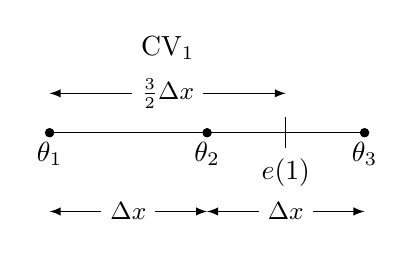
\begin{tikzpicture}[scale=2]
			\tikzset{dimen/.style={<->,>=latex,thin,every rectangle node/.style={fill=white,midway,font=\small}}}
			
			\draw (0,0) -- (2,0);
			
			\draw (1.5, -0.1) -- (1.5, 0.1);
				
			\foreach \i in {0, 1, 2}
				\filldraw (\i, 0) circle (0.75pt);
				
			\node[below] at (0, 0) {$\theta_1$};
			\node[below] at (1, 0) {$\theta_2$};
			\node[below] at (2, 0) {$\theta_3$};
			\node[below] at (1.5, -0.1) {$e(1)$};
			\node[above] at (0.75, 0.4) {CV$_1$};
			
			\draw [dimen] (0, 0.25) -- (1.5, 0.25) node {$\frac{3}{2} \Delta x$};
			\draw [dimen] (0, -0.5) -- (1.0, -0.5) node {$\Delta x$};
			\draw [dimen] (1.0, -0.5) -- (2.0, -0.5) node {$\Delta x$};
		\end{tikzpicture}
		\caption{Left CV}
	\end{subfigure}
	\begin{subfigure}[t]{0.3\textwidth}
		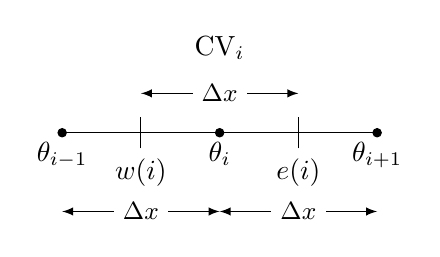
\begin{tikzpicture}[scale=2]
			\tikzset{dimen/.style={<->,>=latex,thin,every rectangle node/.style={fill=white,midway,font=\small}}}
			
			\draw (0,0) -- (2,0);
			
			\foreach \i in {0.5, 1.5}
				\draw (\i, -0.1) -- (\i, 0.1);
			
			\foreach \i in {0, 1, 2}
			\filldraw (\i, 0) circle (0.75pt);
			
			\node[below] at (0, 0) {$\theta_{i-1}$};
			\node[below] at (1, 0) {$\theta_i$};
			\node[below] at (2, 0) {$\theta_{i+1}$};
			\node[below] at (1.5, -0.1) {$e(i)$};
			\node[below] at (0.5, -0.1) {$w(i)$};
			\node[above] at (1.0, 0.4) {CV$_i$};
			
			\draw [dimen] (0.5, 0.25) -- (1.5, 0.25) node {$\Delta x$};
			\draw [dimen] (0, -0.5) -- (1.0, -0.5) node {$\Delta x$};
			\draw [dimen] (1, -0.5) -- (2.0, -0.5) node {$\Delta x$};
		\end{tikzpicture}
		\caption{Interior CV ($1 < i < N - 1)$}
	\end{subfigure}
	\begin{subfigure}[t]{0.3\textwidth}
		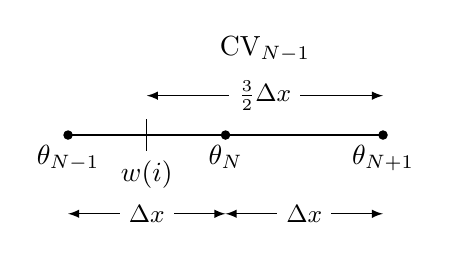
\begin{tikzpicture}[scale=2]
			\tikzset{dimen/.style={<->,>=latex,thin,every rectangle node/.style={fill=white,midway,font=\small}}}
			
			\draw (0,0) -- (2,0);
			
			\draw (0.5, -0.1) -- (0.5, 0.1);
			
			\foreach \i in {0, 1, 2}
			\filldraw (\i, 0) circle (0.75pt);
			
			\node[below] at (0, 0) {$\theta_{N-1}$};
			\node[below] at (1, 0) {$\theta_{N}$};
			\node[below] at (2, 0) {$\theta_{N+1}$};
			\node[below] at (0.5, -0.1) {$w(i)$};
			\node[above] at (1.25, 0.4) {CV$_{N-1}$};
			
			\draw [dimen] (0.5, 0.25) -- (2, 0.25) node {$\frac{3}{2} \Delta x$};
			\draw [dimen] (0, -0.5) -- (1.0, -0.5) node {$\Delta x$};
			\draw [dimen] (1.0, -0.5) -- (2.0, -0.5) node {$\Delta x$};
		\end{tikzpicture}
		\caption{Right CV}
	\end{subfigure}
	\caption{The control volumes defined for discretization of the problem.}
	\label{fig:CVs}
\end{figure}

\subsubsection*{Internal control volume equation}

We start with the integration over an interior control volume, as
\[
	\int_{\text{CV}_i} \left[ -\dv{^2\theta}{x^2} + \frac{hp}{kA} \theta \right] dx = 0\,, \quad 1 < i < N - 1\,,
\]
in which we know that the material properties are independent, to obtain
\[
	- \left( \dv{\theta}{x}\Big|_{e(i)} - \dv{\theta}{x}\Big|_{w(i)} \right) + \frac{hp\Delta x}{kA} \theta_i = 0\,, \quad 1 < i < N - 1\,.
\]
Use the two node formulation for the derivative terms and simplify as
\begin{align}
	- \left( \frac{\theta_{i+1} - \theta_i}{\Delta x} - \frac{\theta_i - \theta_{i - 1}}{\Delta x} \right) + \frac{hp\Delta x}{kA} \theta_i & = 0 \,, \quad 1 < i < N - 1\,,\nonumber \\
	- \frac{1}{\Delta x} \theta_{i-1} + \left(\frac{h p \Delta x}{kA} + \frac{2}{\Delta x}\right) \theta_i - \frac{1}{\Delta x} \theta_{i+1} & = 0\,, \quad 1 < i < N - 1\,.
	\label{eq:int_cv}
\end{align}

\subsubsection*{Left boundary control volume equation}

Utilize Equation \ref{eq:int_cv} for $i = 1$ with a known value of $\theta_1 = T_0 - T_\infty$ to obtain
\begin{equation}
	\left(\frac{h p \Delta x}{kA} + \frac{2}{\Delta x}\right) \theta_1 - \frac{1}{\Delta x} \theta_2 = \frac{1}{\Delta x} (T_0 - T_\infty)\,.
	\label{eq:int_leftcv}
\end{equation}

\subsubsection*{Right boundary control volume equation}

At the right boundary we have
\[
	\dv{\theta}{x} \Big|_{x = 1~\text{m}} = - \frac{k}{h} \theta\,.
\]

Use a backward difference for the derivative term to obtain
\begin{align}
	\frac{\theta_{N+1} - \theta_N}{\frac{1}{2}\Delta x} & = - \frac{h}{k} \theta_{N+1}\,,\nonumber \\
	-\theta_N + \left(1 + \frac{h \Delta x}{2k}\right) \theta_{N+1} & = 0\,.
	\label{eq:int_rightcv}
\end{align}

\subsubsection*{Simplified control volume equations}

First, define
\[
	a_w = a_e = \frac{1}{\Delta x} \quad \text{and} \quad a_p = \frac{h p \Delta x}{kA} + \frac{2}{\Delta x}\,,
\]
in which we are then solving the system 
\begin{equation}
	\begin{cases}
		a_p \theta_1 - a_e \theta_2 = a_w (T_0 - T_\infty)\,, \\
		a_w \theta_{i - 1} - a_p \theta_i + a_e \theta_{i+1} = 0\,, & 1 < i < N - 1\,,\\
		-\theta_N + \left(1 + \frac{h \Delta x}{2k}\right) \theta_{N+1} = 0\,.
	\end{cases}
\end{equation}

\section*{Results}

\begin{figure}[H]
	\centering
	\includegraphics[width=\linewidth]{../python/result}
	\caption{The plotted solution.}
	\label{fig:results}
\end{figure}

\end{document}
